\chapter{REST}

\section{HTTP-verzoekmethoden}

Spring Boot is een goede keuze als je een REST API (of voluit een RESTful web API) wilt ontwikkelen in Java.

REST (Representational State Transfer) is een gestandaardiseerde manier om communicatie tussen verschillende softwaretoepassingen over het internet mogelijk te maken. 
In een RESTful web applicatie wordt de functionaliteit van de applicatie beschikbaar gesteld als resources, die kunnen worden geïdentificeerd door URI's (Uniform Resource Identifiers).  Gebruikers en andere applicaties kunnen met deze resources communiceren via standaard HTTP-verzoekmethoden (HTTP-request, HTTP-method of HTTP-verb). In essentie is HTTP het transportprotocol dat wordt gebruikt om gegevens over te dragen,  terwijl REST de verzameling van ontwerpprincipes is die bepalen hoe die gegevens moeten worden georganiseerd en benaderd.

\begin{itemize}
\item \textbf{GET}: Het GET-verzoek wordt gebruikt om gegevens op te halen van een specifieke resource. 

Voorbeeld URI: GET /api/products/123

Dit verzoek haalt informatie op over het product met ID 123.

\item \textbf{POST}: Het POST-verzoek wordt gebruikt om nieuwe gegevens naar een resource te verzenden. Het wordt vaak gebruikt voor het maken van nieuwe resources of het toevoegen van gegevens aan een bestaande resource.

Voorbeeld URI: POST /api/products

Dit verzoek voegt een nieuw product toe aan de lijst van producten.

\item \textbf{PUT}: Het PUT-verzoek wordt gebruikt om gegevens bij te werken voor een specifieke resource of om een nieuwe resource te maken als deze niet bestaat. Het is idempotent, wat betekent dat meerdere PUT-verzoeken hetzelfde resultaat opleveren.

Voorbeeld URI: PUT /api/products/123

Dit verzoek bijwerken de informatie van het product met ID 123.

\item \textbf{DELETE}: Het DELETE-verzoek wordt gebruikt om een resource te verwijderen of te deactiveren.

Voorbeeld URI: DELETE /api/products/123

Dit verzoek verwijdert het product met ID 123 uit de lijst van producten.
\end{itemize}


\section{De RestController}

Spring boot heeft een annotatie voorzien voor de Java Bean die verantwoordelijk is voor het afhandelen van HTTP requests nl @RestController. Spring boot heeft ook een annotatie @Controller, maar de @RestController zorgt ervoor dat het respons op het HTTP-request automatisch wordt omgezet (geserialiseerd) naar JSON of XML en wordt teruggestuurd naar de client.


\begin{lstlisting}[frame=single]
package be.pxl.demo.api;

import jakarta.annotation.PostConstruct;
import org.springframework.web.bind.annotation.GetMapping;
import org.springframework.web.bind.annotation.RestController;

import java.util.ArrayList;
import java.util.List;
import java.util.Random;

@RestController
@RequestMapping("/greetings")
public class GreetingController {

    private final List<String> messages = new ArrayList<>();
    private static final Random RANDOM = new Random();

    @PostConstruct
    public void init() {
        messages.add("Peek-a-boo!");
        messages.add("Howdy-doody!");
        messages.add("My name's Ralph, and I'm a bad guy.");
        messages.add("I come in peace!");
        messages.add("Put that cookie down!");

    }

    @GetMapping("/hello")
    public String doGreeting() {
        return messages.get(RANDOM.nextInt(messages.size()));
    }
}
\end{lstlisting}

De @RestController markeert de klasse GreetingController als een REST-controller.
De annotatie @RequestMapping("/greetings") specificeert het basispad voor alle requests die door deze controller worden afgehandeld.
@GetMapping("/hello") geeft aan dat de goGreeting-methode wordt uitgevoerd wanneer een HTTP GET-verzoek wordt gemaakt naar het pad "/greetings/hello". Het resultaat van deze methode wordt automatisch omgezet in tekst en teruggestuurd als de respons.

\begin{figure}[H]
  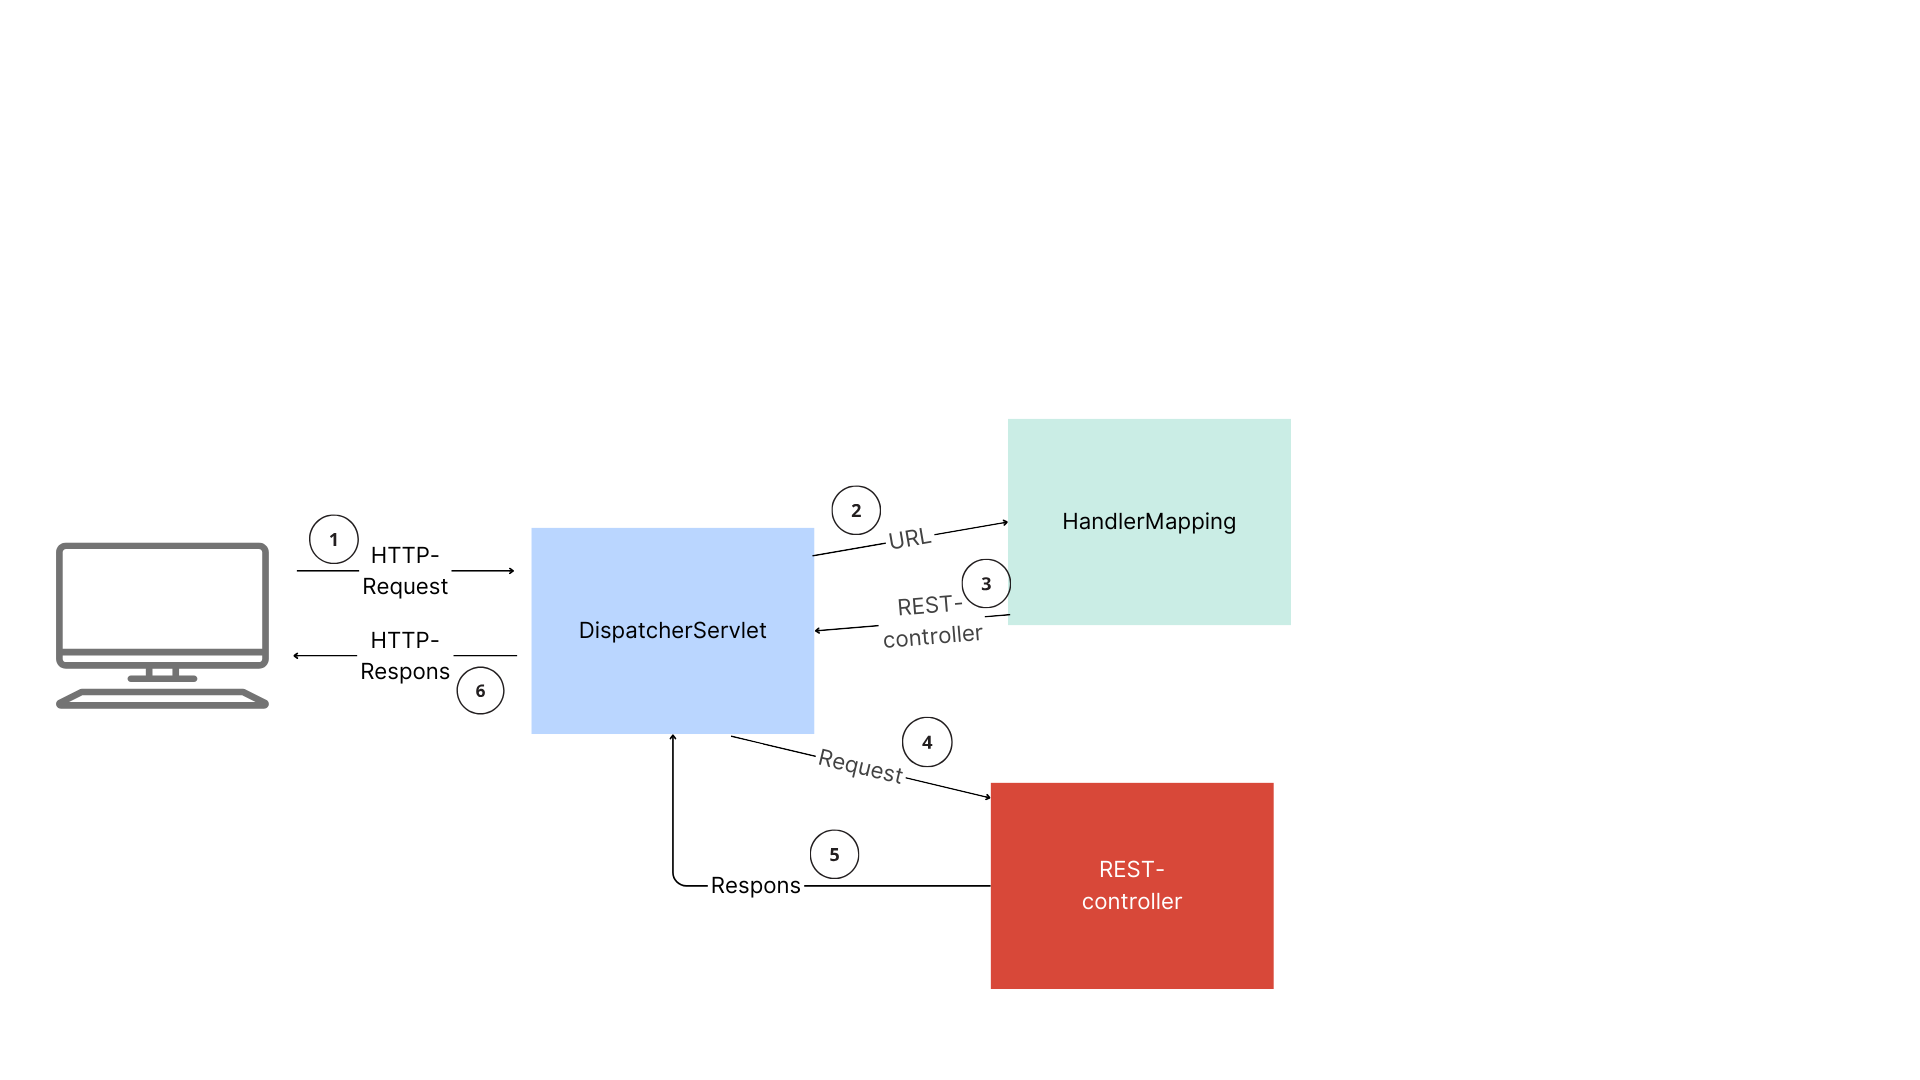
\includegraphics[width=\linewidth]{images/chapter-rest/dispatcherservlet.png}
  \caption{Een REST-verzoek afhandelen}
  \label{fig:test_passed}
\end{figure}

De component van Spring Boot die verantwoordelijk is dat een HTTP-request door de juiste REST-controller wordt afgehandeld is de DispatcherServlet.  De DispatcherServlet is onderdeel van Spring MVC.  De DispatcherServlet bepaalt welke controller een HTTP-request moet afhandelen,  hij geeft het request door aan de juiste controller en  verwerkt het respons van de controller om een HTTP-respons terug te sturen naar de client.

Om te achterhalen welke REST-controller verantwoordelijk is om een HTTP-request af te handelen raadpleegt de DispatcherServlet de HandlerMapping. De HandlerMapping is als het ware een kaart die URL's koppelt aan specifieke controllerklassen en methoden.
Op basis van de URL in het binnenkomende request bepaalt de DispatcherServlet welke controllerklasse en methode verantwoordelijk zijn voor het afhandelen van het request.


\begin{oefening}
Create the package \textit{be.pxl.demo.api}. Add the class \textbf{GreetingController} in this package. Restart the Spring Boot application and open the URL \url{http://localhost:8080/greetings/hello} in a browser. Voeg in de REST-controller een methode toe met de URI GET /greetings/daytime die de huidige dag en het tijdstip teruggeeft in het formaat 'Maandag 18 september 2023'.
\end{oefening}

\section{MusicPlaylist}

We gaan een nieuwe Spring Boot toepassing starten waarmee we een muziek playlist beheren. 

\begin{oefening}
Maak een nieuwe Spring boot toepassing MusicPlaylist. We gebruiken Spring MVC om een RESTful webtoepassing te maken.  
\end{oefening}

\subsection{Een liedje toevoegen aan een playlist}

\begin{apiRoute}{post}{/playlist/songs}{add a new song to the playlist}
\begin{routeParameter}
	\noRouteParameter {no parameter }
\end{routeParameter}
\begin{routeRequest}{application/json}
\begin{routeRequestBody}
{
"name" : " Apfelmus " ,
" count " : 25
}
\end{routeRequestBody}
\end{routeRequest}
\begin{routeResponse}{application/json}
\begin{routeResponseItem}{200}{ ok}
\begin{ routeResponseItemBody }
{
" i d " : 8 6 7 6 5 4 6 7 8 ,
"name" : " Apfelmus " ,
" count " : 25
}
\end{routeResponseItemBody}
\end{routeResponseItem}
\end{routeResponse}
\end{apiRoute}


@Service
public class MusicPlaylistService {

    public String calculatePlaylistDuration(List<String> songDurations) {
        int totalSeconds = 0;

        for (String duration : songDurations) {
            String[] parts = duration.split(":");
            if (parts.length == 2) {
                int minutes = Integer.parseInt(parts[0]);
                int seconds = Integer.parseInt(parts[1]);
                totalSeconds += (minutes * 60) + seconds;
            }
        }

        int hours = totalSeconds / 3600;
        int remainingSeconds = totalSeconds % 3600;
        int minutes = remainingSeconds / 60;
        int seconds = remainingSeconds % 60;

        return String.format("%d:%02d:%02d", hours, minutes, seconds);
    }
}


Certainly, here's an example of a Song class in Java with attributes for the artist, duration (in seconds), title, and an optional album attribute:

java
Copy code
public class Song {
    private String artist;
    private int durationInSeconds;
    private String title;
    private String album;

    public Song(String artist, int durationInSeconds, String title) {
        this.artist = artist;
        this.durationInSeconds = durationInSeconds;
        this.title = title;
    }

    public Song(String artist, int durationInSeconds, String title, String album) {
        this(artist, durationInSeconds, title);
        this.album = album;
    }

    public String getArtist() {
        return artist;
    }

    public int getDurationInSeconds() {
        return durationInSeconds;
    }

    public String getTitle() {
        return title;
    }

    public String getAlbum() {
        return album;
    }

    public void setAlbum(String album) {
        this.album = album;
    }

    @Override
    public String toString() {
        return "Song{" +
                "artist='" + artist + '\'' +
                ", durationInSeconds=" + durationInSeconds +
                ", title='" + title + '\'' +
                ", album='" + album + '\'' +
                '}';
    }
}
In this Song class:

The artist, durationInSeconds, and title are required attributes and are set via the constructor.
The album attribute is optional and can be set separately using a setter method.
Getter methods are provided to retrieve the values of the attributes.
A toString method is overridden to provide a human-readable representation of the Song object.
You can customize this class further or add more attributes and methods based on your specific requirements. This basic structure allows you to create and work with Song objects, storing information about artists, song titles, durations, and albums.




User
Can a spring boot class MusicPlaylistService with annotation @Service maintain a List<Song> myPlaylist. I want to add a method to add, remove a song and calculate the duration of the playlist. What is the scope of the list.
ChatGPT
Yes, you can certainly have a Spring Boot service class, like MusicPlaylistService, maintain a List<Song> (e.g., myPlaylist) to add, remove songs, and calculate the duration of the playlist. The scope of the list can be configured as either a singleton or a prototype, depending on your requirements.

Singleton Scope (Default): If you annotate the MusicPlaylistService with @Service without specifying a scope, the service will be a singleton by default. This means that there will be only one instance of MusicPlaylistService throughout the lifetime of your Spring Boot application, and the myPlaylist list will be shared among all users or requests accessing this service. This can be a good choice if you want to maintain a single, shared playlist for all users or sessions.
Example:

java
Copy code
@Service
public class MusicPlaylistService {
    private List<Song> myPlaylist = new ArrayList<>();

    // Add, remove, and calculate duration methods
}
Prototype Scope: If you want each request or user to have its own instance of MusicPlaylistService with a separate playlist, you can configure the service with a prototype scope. To do this, you can use the @Scope annotation with the ConfigurableBeanFactory.SCOPE\_PROTOTYPE value.
Example:

With this configuration, Spring will create a new instance of MusicPlaylistService for each request or usage, and each instance will have its own isolated myPlaylist. This is useful if you want to maintain separate playlists for different users or sessions.

Choose the scope that best fits your application's requirements. If you want a single shared playlist for all users, the default singleton scope is suitable. If you need separate playlists for different users, consider using the prototype scope as shown in the second example.


 